\begin{center}
    \captionof{figure}{Within- and Between-Person Effects of Continuous Predictor and Outcome}

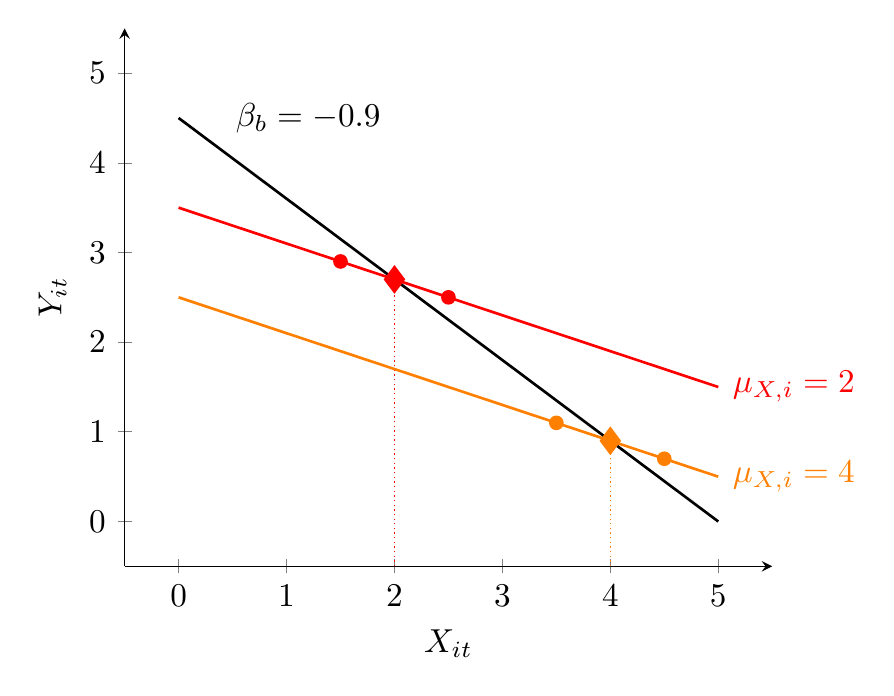
\begin{tikzpicture}[scale=1.2]
    \begin{axis}[
        axis x line=left, 
        axis y line=left, 
        xlabel={$X_{it}$}, ylabel={$Y_{it}$},
        xmin=0, xmax=5, ymin=0, ymax=5,
        xtick={0,1,2,3,4,5},
        ytick={0,1,2,3,4,5},
        enlargelimits=true,
        clip=false,
        xshift=-15mm
    ]

    \pgfmathsetmacro{\gammaZero}{4.5}
    \pgfmathsetmacro{\gammaOne}{-0.5}
    \pgfmathsetmacro{\betaOne}{-0.4}
    \pgfmathsetmacro{\betaB}{-0.9}  % gamma01 + beta1

    % === Within-person: mu_X = 2 ===
    \addplot[domain=0:5, thick, red] {\gammaZero + \gammaOne*2 + \betaOne*x};
    \addplot[only marks, red] coordinates {
        (1.5, {4.5 - 0.5*2 - 0.4*1.5})
        % (2.0, {4.5 - 0.5*2 - 0.4*2.0})
        (2.5, {4.5 - 0.5*2 - 0.4*2.5})
    };
    \addplot[only marks, mark=diamond*, mark size=4pt, red] coordinates {
        (2.0, {4.5 - 0.5*2 - 0.4*2.0})
    };
    \addplot[densely dotted, thin, red] coordinates {
        (2.0, -0.5)
        (2.0, {4.5 - 0.5*2 - 0.4*2.0})
    };

    % === Within-person: mu_X = 4 ===
    \addplot[domain=0:5, thick, orange] {\gammaZero + \gammaOne*4 + \betaOne*x};
    \addplot[only marks, orange] coordinates {
        (3.5, {4.5 - 0.5*4 - 0.4*3.5})
        % (4.0, {4.5 - 0.5*4 - 0.4*4.0})
        (4.5, {4.5 - 0.5*4 - 0.4*4.5})
    };
    \addplot[only marks, mark=diamond*, mark size=4pt, orange] coordinates {
        (4.0, {4.5 - 0.5*4 - 0.4*4.0})
    };
    \addplot[densely dotted, thin, orange] coordinates {
        (4.0, -0.5)
        (4.0, {4.5 - 0.5*4 - 0.4*4.0})
    };

    % === Between-person regression line ===
    \addplot[thick, black, domain=0:5] {\gammaZero + \betaB*x};

    % === Labels ===
    \node[red] at (axis cs:5.7,1.5) {$\mu_{X,i}=2$};
    \node[orange] at (axis cs:5.7,0.5) {$\mu_{X,i}=4$};
    \node[black] at (axis cs:1.2,4.5) {$\beta_\text{b} = -0.9$};

    \end{axis}
\end{tikzpicture}

    \label{fig:withinbetween-contxy}
    \begin{figurenote}
        The solid black slope represents the between-person effect and the colored slopes the within-cluster effects. The X-axis simultaneously represents $X_{it}$ for the within-slope and $\mu_{X,i}$ for the between-slope; and the Y-axis represents $Y_{it}$ for the within slope and $Y_i$ for the between-slope. Dots reflect possible datapoints and diamonds reflect the position of $\mu_{X,i}$ on the within-person slope.
    \end{figurenote}
\end{center}